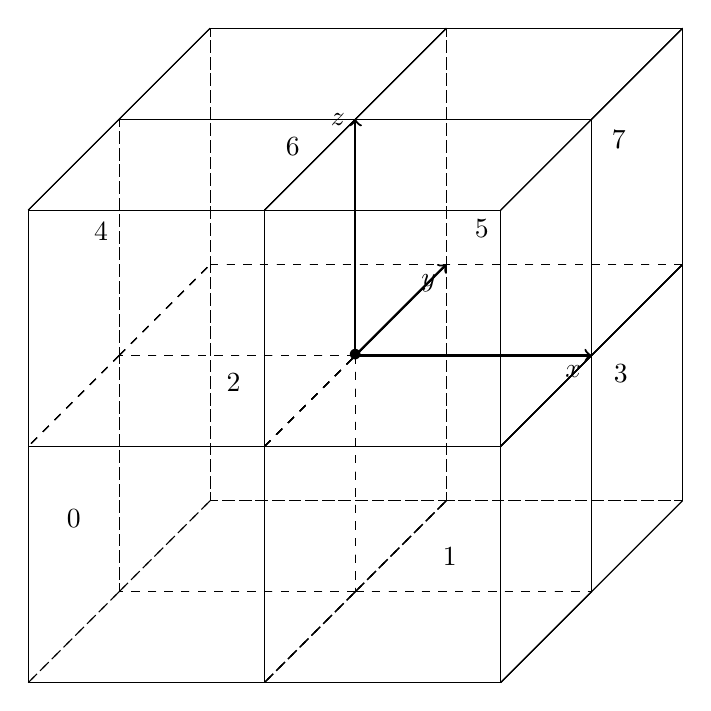
\begin{tikzpicture}[scale = 3, cm={1,0,-1,-1, (0,0)},y=-3.85mm, z = -1cm]
    \draw[thick,->,black] (0,0,0) -- (1,0,0) node[anchor=north east]{$x$};
    \draw[thick,->] (0,0,0) -- (0,1,0) node[anchor=north east]{$y$};
    \draw[thick,->] (0,0,0) -- (0,0,1) node[anchor=east]{$z$};

\node at (0,0,0) {$\bullet$};
\node at (1.2,-0.2,0) {$3$};
\node at (0.4,0,-0.85) {$1$};
\node at (0.15,1,0.15) {$5$};
\node at (1,0.3,0.8)  {$7$};
\node at (-0.4,-0.3,0){$2$};
\node at (-1,-0.2,0.6){$4$};
\node at (-1,-0.5,-0.5){$0$};
\node at (-0.65,1,0.5) {$6$};

%Cube Left Front Upper

%X-Y rectangle Z = 1
\draw[] (-1,-1,1) -- (0,-1,1);
\draw[] (0,-1,1)  -- (0,0,1);
\draw[] (0,0,1)   -- (-1,0,1);
\draw[] (-1,0,1)  -- (-1,-1,1);

%X-Z rectangle Y = -1
\draw[] (-1,-1,1) -- (-1,-1,0);
\draw[] (-1,-1,0) -- (0,-1,0);
\draw[] (0,-1,0)  -- (0,-1,1);
\draw[] (0,-1,1)  -- (-1,-1,1);

%Z-Y rectangle X = 0
\draw[] (0,-1,1) -- (0,-1,0);
\draw[dashed] (0,-1,0) -- (0,0,0);
\draw[dashed] (0,0,0)  -- (0,0,1);
\draw[]  (0,0,1) -- (0,-1,1);

%X-Y rectangle Z = 0
\draw[] (-1,-1,0) -- (0,-1,0);
\draw[dashed] (0,-1,0) -- (0,0,0);
\draw[dashed] (0,0,0)  -- (-1,0,0);
\draw[dashed] (-1,0,0) -- (-1,-1,0);

%Y-Z rectangle X = -1
\draw[] (-1,-1,0) -- (-1,-1,1);
\draw[] (-1,-1,1) -- (-1,0,1);
\draw[dashed] (-1,0,1) -- (-1,0,0);
\draw[dashed] (-1,0,0) -- (-1,-1,0);

%X-Z rectangle Y = 0
\draw[dashed] (0,0,0)  -- (-1,0,0);
\draw[dashed] (-1,0,0) -- (-1,0,1);
\draw[dashed] (0,0,0)  -- (0,0,1);
\draw[]       (0,0,1)  -- (-1,0,1);



%Cube Right Front Upper

%X-Y rectangle Z = 1
\draw[] (1,-1,1) -- (0,-1,1);
\draw[] (0,-1,1)  -- (0,0,1);
\draw[] (0,0,1)   -- (1,0,1);
\draw[] (1,0,1)  -- (1,-1,1);

%rX-Z rectangle Y = -1
\draw[] (1,-1,1) -- (1,-1,0);
\draw[] (1,-1,0) -- (0,-1,0);
\draw[] (0,-1,0)  -- (0,-1,1);
\draw[] (0,-1,1)  -- (1,-1,1);

%Y-Z rectangle X = 0
\draw[] (0,-1,1) -- (0,-1,0);
\draw[dashed] (0,-1,0) -- (0,0,0);
\draw[dashed] (0,0,0)  -- (0,0,1);
\draw[]  (0,0,1) -- (0,-1,1);

%X-Y rectangle Z = 0
\draw[] (1,-1,0) -- (0,-1,0);
\draw[dashed] (0,-1,0) -- (0,0,0);
\draw[dashed] (0,0,0)  -- (1,0,0);
\draw[] (1,0,0) -- (1,-1,0);

%Y-Z rectangle X = 1
\draw[] (1,-1,0) -- (1,-1,1);
\draw[] (1,-1,1) -- (1,0,1);
\draw[] (1,0,1) -- (1,0,0);
\draw[] (1,0,0) -- (1,-1,0);

%X-Z rectangle Y = 0
\draw[dashed] (0,0,0)  -- (1,0,0);
\draw[] (1,0,0) -- (1,0,1);
\draw[dashed] (0,0,0)  -- (0,0,1);
\draw[]       (0,0,1)  -- (1,0,1);



%Cube Right Back Upper

%X-Y rectangle Z = 1
\draw[] (1,1,1) -- (0,1,1);
\draw[] (0,1,1)  -- (0,0,1);
\draw[] (0,0,1)   -- (1,0,1);
\draw[] (1,0,1)  -- (1,1,1);

%X-Z rectangle Y = 1
\draw[] (1,1,1) -- (1,1,0);
\draw[dashed] (1,1,0) -- (0,1,0);
\draw[dashed] (0,1,0)  -- (0,1,1);
\draw[] (0,1,1)  -- (1,1,1);

%Y-Z rectangle X = 0
\draw[dashed] (0,1,1) -- (0,1,0);
\draw[dashed] (0,1,0) -- (0,0,0);
\draw[dashed] (0,0,0)  -- (0,0,1);
\draw[]  (0,0,1) -- (0,1,1);

%X-Y rectangle Z = 0
\draw[dashed] (1,1,0) -- (0,1,0);
\draw[dashed] (0,1,0) -- (0,0,0);
\draw[dashed] (0,0,0)  -- (1,0,0);
\draw[] (1,0,0) -- (1,1,0);

%Y-Z rectangle X = 1
\draw[] (1,1,0) -- (1,1,1);
\draw[] (1,1,1) -- (1,0,1);
\draw[] (1,0,1) -- (1,0,0);
\draw[] (1,0,0) -- (1,1,0);

%X-Z rectangle Y = 0
\draw[dashed] (0,0,0)  -- (1,0,0);
\draw[] (1,0,0) -- (1,0,1);
\draw[dashed] (0,0,0)  -- (0,0,1);
\draw[]       (0,0,1)  -- (1,0,1);


%Cube Left Back Upper

%X-Y rectangle Z = 1
\draw[] (-1,1,1) -- (0,1,1);
\draw[] (0,1,1)  -- (0,0,1);
\draw[] (0,0,1)   -- (-1,0,1);
\draw[] (-1,0,1)  -- (-1,1,1);

%X-Z rectangle Y = 1
\draw[dashed] (-1,1,1) -- (-1,1,0);
\draw[dashed] (-1,1,0) -- (0,1,0);
\draw[dashed] (0,1,0)  -- (0,1,1);
\draw[] (0,1,1)  -- (-1,1,1);

%Y-Z rectangle X = 0
\draw[dashed] (0,1,1) -- (0,1,0);
\draw[dashed] (0,1,0) -- (0,0,0);
\draw[dashed] (0,0,0)  -- (0,0,1);
\draw[]  (0,0,1) -- (0,1,1);

%X-Y rectangle Z = 0
\draw[dashed] (-1,1,0) -- (0,1,0);
\draw[dashed] (0,1,0) -- (0,0,0);
\draw[dashed] (0,0,0)  -- (-1,0,0);
\draw[dashed] (-1,0,0) -- (-1,1,0);

%Y-Z rectangle X = -1
\draw[dashed] (-1,1,0) -- (-1,1,1);
\draw[] (-1,1,1) -- (-1,0,1);
\draw[dashed] (-1,0,1) -- (-1,0,0);
\draw[dashed] (-1,0,0) -- (-1,1,0);

%X-Z rectangle Y = 0
\draw[dashed] (0,0,0)  -- (-1,0,0);
\draw[dashed] (-1,0,0) -- (-1,0,1);
\draw[dashed] (0,0,0)  -- (0,0,1);
\draw[]       (0,0,1)  -- (-1,0,1);


%Cube Left Front Lower

%X-Y rectangle Z = -1
\draw[] (-1,-1,-1) -- (0,-1,-1);
\draw[dashed] (0,-1,-1)  -- (0,0,-1);
\draw[dashed] (0,0,-1)   -- (-1,0,-1);
\draw[dashed] (-1,0,-1)  -- (-1,-1,-1);

%X-Z rectangle Y = -1
\draw[] (-1,-1,-1) -- (-1,-1,0);
\draw[] (-1,-1,0) -- (0,-1,0);
\draw[] (0,-1,0)  -- (0,-1,-1);
\draw[] (0,-1,-1)  -- (-1,-1,-1);

%Z-Y rectangle X = 0
\draw[] (0,-1,-1) -- (0,-1,0);
\draw[dashed] (0,-1,0) -- (0,0,0);
\draw[dashed] (0,0,0)  -- (0,0,-1);
\draw[dashed]  (0,0,-1) -- (0,-1,-1);

%X-Y rectangle Z = 0
\draw[] (-1,-1,0) -- (0,-1,0);
\draw[dashed] (0,-1,0) -- (0,0,0);
\draw[dashed] (0,0,0)  -- (-1,0,0);
\draw[dashed] (-1,0,0) -- (-1,-1,0);

%Y-Z rectangle X = -1
\draw[] (-1,-1,0) -- (-1,-1,-1);
\draw[dashed] (-1,-1,-1) -- (-1,0,-1);
\draw[dashed] (-1,0,-1) -- (-1,0,0);
\draw[dashed] (-1,0,0) -- (-1,-1,0);

%X-Z rectangle Y = 0
\draw[dashed] (0,0,0)  -- (-1,0,0);
\draw[dashed] (-1,0,0) -- (-1,0,-1);
\draw[dashed] (0,0,0)  -- (0,0,-1);
\draw[dashed]       (0,0,-1)  -- (-1,0,-1);



%Cube Right Front Lower

%X-Y rectangle Z = -1
\draw[] (1,-1,-1) -- (0,-1,-1);
\draw[dashed] (0,-1,-1)  -- (0,0,-1);
\draw[dashed] (0,0,-1)   -- (1,0,-1);
\draw[] (1,0,-1)  -- (1,-1,-1);

%rX-Z rectangle Y = -1
\draw[] (1,-1,-1) -- (1,-1,0);
\draw[] (1,-1,0) -- (0,-1,0);
\draw[] (0,-1,0)  -- (0,-1,-1);
\draw[] (0,-1,-1)  -- (1,-1,-1);

%Y-Z rectangle X = 0
\draw[] (0,-1,-1) -- (0,-1,0);
\draw[dashed] (0,-1,0) -- (0,0,0);
\draw[dashed] (0,0,0)  -- (0,0,-1);
\draw[dashed]  (0,0,-1) -- (0,-1,-1);

%X-Y rectangle Z = 0
\draw[] (1,-1,0) -- (0,-1,0);
\draw[dashed] (0,-1,0) -- (0,0,0);
\draw[dashed] (0,0,0)  -- (1,0,0);
\draw[] (1,0,0) -- (1,-1,0);

%Y-Z rectangle X = 1
\draw[] (1,-1,0) -- (1,-1,-1);
\draw[] (1,-1,-1) -- (1,0,-1);
\draw[] (1,0,-1) -- (1,0,0);
\draw[] (1,0,0) -- (1,-1,0);

%X-Z rectangle Y = 0
\draw[dashed] (0,0,0)  -- (1,0,0);
\draw[] (1,0,0) -- (1,0,-1);
\draw[dashed] (0,0,0)  -- (0,0,-1);
\draw[dashed] (0,0,-1)  -- (1,0,-1);



%Cube Right Back Lower

%X-Y rectangle Z = -1
\draw[dashed] (1,1,-1) -- (0,1,-1);
\draw[dashed] (0,1,-1)  -- (0,0,-1);
\draw[dashed] (0,0,-1)   -- (1,0,-1);
\draw[] (1,0,-1)  -- (1,1,-1);

%X-Z rectangle Y = 1
\draw[] (1,1,-1) -- (1,1,0);
\draw[dashed] (1,1,0) -- (0,1,0);
\draw[dashed] (0,1,0)  -- (0,1,-1);
\draw[dashed] (0,1,-1)  -- (1,1,-1);

%Y-Z rectangle X = 0
\draw[dashed] (0,1,1) -- (0,1,0);
\draw[dashed] (0,1,0) -- (0,0,0);
\draw[dashed] (0,0,0)  -- (0,0,-1);
\draw[dashed]  (0,0,-1) -- (0,1,-1);

%X-Y rectangle Z = 0
\draw[dashed] (1,1,0) -- (0,1,0);
\draw[dashed] (0,1,0) -- (0,0,0);
\draw[dashed] (0,0,0)  -- (1,0,0);
\draw[] (1,0,0) -- (1,1,0);

%Y-Z rectangle X = 1
\draw[] (1,1,0) -- (1,1,1);
\draw[] (1,1,1) -- (1,0,1);
\draw[] (1,0,1) -- (1,0,0);
\draw[] (1,0,0) -- (1,1,0);

%X-Z rectangle Y = 0
\draw[dashed] (0,0,0)  -- (1,0,0);
\draw[] (1,0,0) -- (1,0,-1);
\draw[dashed] (0,0,0)  -- (0,0,-1);
\draw[dashed]       (0,0,-1)  -- (1,0,-1);


%Cube Left Back Lower

%X-Y rectangle Z = -1
\draw[dashed] (-1,1,-1) -- (0,1,-1);
\draw[dashed] (0,1,-1)  -- (0,0,-1);
\draw[dashed] (0,0,-1)   -- (-1,0,-1);
\draw[dashed] (-1,0,-1)  -- (-1,1,-1);

%X-Z rectangle Y = 1
\draw[dashed] (-1,1,-1) -- (-1,1,0);
\draw[dashed] (-1,1,0) -- (0,1,0);
\draw[dashed] (0,1,0)  -- (0,1,-1);
\draw[dashed] (0,1,-1)  -- (-1,1,-1);

%Y-Z rectangle X = 0
\draw[dashed] (0,1,-1) -- (0,1,0);
\draw[dashed] (0,1,0) -- (0,0,0);
\draw[dashed] (0,0,0)  -- (0,0,-1);
\draw[dashed]  (0,0,-1) -- (0,1,-1);

%X-Y rectangle Z = 0
\draw[dashed] (-1,1,0) -- (0,1,0);
\draw[dashed] (0,1,0) -- (0,0,0);
\draw[dashed] (0,0,0)  -- (-1,0,0);
\draw[dashed] (-1,0,0) -- (-1,1,0);

%Y-Z rectangle X = -1
\draw[dashed] (-1,1,0) -- (-1,1,-1);
\draw[dashed] (-1,1,-1) -- (-1,0,-1);
\draw[dashed] (-1,0,-1) -- (-1,0,0);
\draw[dashed] (-1,0,0) -- (-1,1,0);

%X-Z rectangle Y = 0
\draw[dashed] (0,0,0)  -- (-1,0,0);
\draw[dashed] (-1,0,0) -- (-1,0,-1);
\draw[dashed] (0,0,0)  -- (0,0,-1);
\draw[dashed]       (0,0,-1)  -- (-1,0,-1);










\end{tikzpicture}
